\documentclass[a4paper,12pt,twoside]{memoir}

% Castellano
\usepackage[spanish,es-tabla]{babel}
\selectlanguage{spanish}
\usepackage[utf8]{inputenc}
\usepackage[T1]{fontenc}
\usepackage{lmodern} % scalable font
\usepackage{microtype}
\usepackage{placeins}

\RequirePackage{booktabs}
\RequirePackage[table]{xcolor}
\RequirePackage{xtab}
\RequirePackage{multirow}

% Links
\PassOptionsToPackage{hyphens}{url}\usepackage[colorlinks]{hyperref}
\hypersetup{
	allcolors = {red}
}

% Ecuaciones
\usepackage{amsmath}

% Rutas de fichero / paquete
\newcommand{\ruta}[1]{{\sffamily #1}}

% Párrafos
\nonzeroparskip

% Huérfanas y viudas
\widowpenalty100000
\clubpenalty100000

% Evitar solapes en el header
\nouppercaseheads

% Imagenes
\usepackage{graphicx}
\newcommand{\imagen}[2]{
	\begin{figure}[!h]
		\centering
		\includegraphics[width=0.9\textwidth]{#1}
		\caption{#2}\label{fig:#1}
	\end{figure}
	\FloatBarrier
}

\newcommand{\imagenflotante}[2]{
	\begin{figure}%[!h]
		\centering
		\includegraphics[width=0.9\textwidth]{#1}
		\caption{#2}\label{fig:#1}
	\end{figure}
}



% El comando \figura nos permite insertar figuras comodamente, y utilizando
% siempre el mismo formato. Los parametros son:
% 1 -> Porcentaje del ancho de página que ocupará la figura (de 0 a 1)
% 2 --> Fichero de la imagen
% 3 --> Texto a pie de imagen
% 4 --> Etiqueta (label) para referencias
% 5 --> Opciones que queramos pasarle al \includegraphics
% 6 --> Opciones de posicionamiento a pasarle a \begin{figure}
\newcommand{\figuraConPosicion}[6]{%
  \setlength{\anchoFloat}{#1\textwidth}%
  \addtolength{\anchoFloat}{-4\fboxsep}%
  \setlength{\anchoFigura}{\anchoFloat}%
  \begin{figure}[#6]
    \begin{center}%
      \Ovalbox{%
        \begin{minipage}{\anchoFloat}%
          \begin{center}%
            \includegraphics[width=\anchoFigura,#5]{#2}%
            \caption{#3}%
            \label{#4}%
          \end{center}%
        \end{minipage}
      }%
    \end{center}%
  \end{figure}%
}

%
% Comando para incluir imágenes en formato apaisado (sin marco).
\newcommand{\figuraApaisadaSinMarco}[5]{%
  \begin{figure}%
    \begin{center}%
    \includegraphics[angle=90,height=#1\textheight,#5]{#2}%
    \caption{#3}%
    \label{#4}%
    \end{center}%
  \end{figure}%
}
% Para las tablas
\newcommand{\otoprule}{\midrule [\heavyrulewidth]}
%
% Nuevo comando para tablas pequeñas (menos de una página).
\newcommand{\tablaSmall}[5]{%
 \begin{table}
  \begin{center}
   \rowcolors {2}{gray!35}{}
   \begin{tabular}{#2}
    \toprule
    #4
    \otoprule
    #5
    \bottomrule
   \end{tabular}
   \caption{#1}
   \label{tabla:#3}
  \end{center}
 \end{table}
}

%
%Para el float H de tablaSmallSinColores
\usepackage{float}

%
% Nuevo comando para tablas pequeñas (menos de una página).
\newcommand{\tablaSmallSinColores}[5]{%
 \begin{table}[H]
  \begin{center}
   \begin{tabular}{#2}
    \toprule
    #4
    \otoprule
    #5
    \bottomrule
   \end{tabular}
   \caption{#1}
   \label{tabla:#3}
  \end{center}
 \end{table}
}

\newcommand{\tablaApaisadaSmall}[5]{%
\begin{landscape}
  \begin{table}
   \begin{center}
    \rowcolors {2}{gray!35}{}
    \begin{tabular}{#2}
     \toprule
     #4
     \otoprule
     #5
     \bottomrule
    \end{tabular}
    \caption{#1}
    \label{tabla:#3}
   \end{center}
  \end{table}
\end{landscape}
}

%
% Nuevo comando para tablas grandes con cabecera y filas alternas coloreadas en gris.
\newcommand{\tabla}[6]{%
  \begin{center}
    \tablefirsthead{
      \toprule
      #5
      \otoprule
    }
    \tablehead{
      \multicolumn{#3}{l}{\small\sl continúa desde la página anterior}\\
      \toprule
      #5
      \otoprule
    }
    \tabletail{
      \hline
      \multicolumn{#3}{r}{\small\sl continúa en la página siguiente}\\
    }
    \tablelasttail{
      \hline
    }
    \bottomcaption{#1}
    \rowcolors {2}{gray!35}{}
    \begin{xtabular}{#2}
      #6
      \bottomrule
    \end{xtabular}
    \label{tabla:#4}
  \end{center}
}

%
% Nuevo comando para tablas grandes con cabecera.
\newcommand{\tablaSinColores}[6]{%
  \begin{center}
    \tablefirsthead{
      \toprule
      #5
      \otoprule
    }
    \tablehead{
      \multicolumn{#3}{l}{\small\sl continúa desde la página anterior}\\
      \toprule
      #5
      \otoprule
    }
    \tabletail{
      \hline
      \multicolumn{#3}{r}{\small\sl continúa en la página siguiente}\\
    }
    \tablelasttail{
      \hline
    }
    \bottomcaption{#1}
    \begin{xtabular}{#2}
      #6
      \bottomrule
    \end{xtabular}
    \label{tabla:#4}
  \end{center}
}

%
% Nuevo comando para tablas grandes sin cabecera.
\newcommand{\tablaSinCabecera}[5]{%
  \begin{center}
    \tablefirsthead{
      \toprule
    }
    \tablehead{
      \multicolumn{#3}{l}{\small\sl continúa desde la página anterior}\\
      \hline
    }
    \tabletail{
      \hline
      \multicolumn{#3}{r}{\small\sl continúa en la página siguiente}\\
    }
    \tablelasttail{
      \hline
    }
    \bottomcaption{#1}
  \begin{xtabular}{#2}
    #5
   \bottomrule
  \end{xtabular}
  \label{tabla:#4}
  \end{center}
}



\definecolor{cgoLight}{HTML}{EEEEEE}
\definecolor{cgoExtralight}{HTML}{FFFFFF}

%
% Nuevo comando para tablas grandes sin cabecera.
\newcommand{\tablaSinCabeceraConBandas}[5]{%
  \begin{center}
    \tablefirsthead{
      \toprule
    }
    \tablehead{
      \multicolumn{#3}{l}{\small\sl continúa desde la página anterior}\\
      \hline
    }
    \tabletail{
      \hline
      \multicolumn{#3}{r}{\small\sl continúa en la página siguiente}\\
    }
    \tablelasttail{
      \hline
    }
    \bottomcaption{#1}
    \rowcolors[]{1}{cgoExtralight}{cgoLight}

  \begin{xtabular}{#2}
    #5
   \bottomrule
  \end{xtabular}
  \label{tabla:#4}
  \end{center}
}




\graphicspath{ {./img/} }

% Capítulos
\chapterstyle{bianchi}
\newcommand{\capitulo}[2]{
	\setcounter{chapter}{#1}
	\setcounter{section}{0}
	\chapter*{#2}
	\addcontentsline{toc}{chapter}{#2}
	\markboth{#2}{#2}
}

% Apéndices
\renewcommand{\appendixname}{Apéndice}
\renewcommand*\cftappendixname{\appendixname}

\newcommand{\apendice}[1]{
	%\renewcommand{\thechapter}{A}
	\chapter{#1}
}

\renewcommand*\cftappendixname{\appendixname\ }

% Formato de portada
\makeatletter
\usepackage{xcolor}
\newcommand{\tutor}[1]{\def\@tutor{#1}}
\newcommand{\course}[1]{\def\@course{#1}}
\definecolor{cpardoBox}{HTML}{E6E6FF}
\def\maketitle{
  \null
  \thispagestyle{empty}
  % Cabecera ----------------
\noindent
\includegraphics[width=\textwidth]{cabecera}\vspace{1cm}%
  \vfill
  % Título proyecto y escudo informática ----------------
  \colorbox{cpardoBox}{%
    \begin{minipage}{.8\textwidth}
      \vspace{.5cm}\Large
      \begin{center}
      \textbf{TFG del Grado en Ingeniería Informática}\vspace{.6cm}\\
      \textbf{\LARGE\@title{}}
      \end{center}
      \vspace{.2cm}
    \end{minipage}

  }%
  \hfill\begin{minipage}{.20\textwidth}
    
\includegraphics[width=\textwidth]{escudoInfor}
  \end{minipage}
  \vfill
  % Datos de alumno, curso y tutores ------------------
  \begin{center}%
  {%
    \noindent\LARGE
    Presentado por \@author{}\\ 
    en Universidad de Burgos --- \@date{}\\
    Tutor: \@tutor{}\\
  }%
  \end{center}%
  \null
  \cleardoublepage
  }
\makeatother

\newcommand{\nombre}{Diana Bringas Ochoa}
\newcommand{\nombreTFG}{GII 20.09 Herramienta web repositorios de TFGII}

% Datos de portada
\title{\nombreTFG \\Documentación Técnica}
\author{Diana Bringas Ochoa}
\tutor{Álvar Arnaiz González y Carlos López Nozal}
\date{\today}

\begin{document}

\maketitle



\cleardoublepage



%%%%%%%%%%%%%%%%%%%%%%%%%%%%%%%%%%%%%%%%%%%%%%%%%%%%%%%%%%%%%%%%%%%%%%%%%%%%%%%%%%%%%%%%



\frontmatter


\clearpage

% Indices
\tableofcontents

\clearpage

\listoffigures

\clearpage

\listoftables

\clearpage

\mainmatter

\appendix

\apendice{Plan de Proyecto Software}

\section{Introducción}
En esta sección se detallará la planificación que se ha realizado, el estudio de viabilidad tanto de la parte económica como de la legal.

\section{Planificación temporal}
\subsection{Sprint 0 (26/10/2019 - 25/11/2019)}
Puesta a punto del proyecto, planteamiento de las herramientas con las que trabajar, búsqueda de alternativas y toma de contacto con las herramientas nuevas que se van a emplear.
Las tareas que se realizaron fueron:
\begin{itemize}
	\tightlist
	\item Añadir la extensión ZenHub al navegador. 
	\item Clonar el repositorio en local. 
	\item Investigar sobre Vaadin.
	\item Actualización del README.md 
	\item Investigar LaTeX
\end{itemize}

\subsection{Sprint 1 (25/11/2020 - )}
Generación de test unitarios, búsqueda de trabajos similares, cambio del driver para conectarse con el excel, información para obtener ideas de como realizar ciertas mejoras y comienzo de la documentación del proyecto. Mejora de la cobertura de la aplicación web.

Las tareas planteadas fueron:
\begin{itemize}
	\tightlist
	\item Instalación Miktex + TexStudio
	\item Se comienza la documentación en LaTeX  - Spring 0
	\item Generar nuevos test
	\item Cambiar driver JDBC 
\end{itemize}

\section{Estudio de viabilidad}
\subsection{Viabilidad económica}
En este apartado se detallan los costes que llevaría realizar este proyecto.

\subsubsection{Coste del personal}

\subsubsection{Coste hardware}
Referente a los costes del equipo utilizado en el desarrollo del trabajo. Teniendo en cuenta el precio del ordenador empleado de aproximadamente 700 euros.

\subsubsection{Coste software}
Referente a los costes de las herramientas software no gratuitas empleadas en el proyecto. Como es el caso del Sistema Operativo Windows o el Microsoft Office 365.

\subsection{Viabilidad legal}
En este apartado se detallaran las licencias de cada dependencia que se ha utilizado en el proyecto

\tablaSmallSinColores{Dependencias del proyecto}{ l | l | l }{dependencias}
{\textbf{Software} & \textbf{Licencia} \\}{
	Vaadin & Apache License 2.0 \\
	Vaadin Maven Plugin & Apache License 2.0 \\
}
\apendice{Especificación de Requisitos}

\section{Introducción}

\section{Objetivos generales}

\section{Catalogo de requisitos}

\section{Especificación de requisitos}



\apendice{Especificación de diseño}

\section{Introducción}

\section{Diseño de datos}

\section{Diseño procedimental}

\section{Diseño arquitectónico}



\apendice{Documentación técnica de programación}

\section{Introducción}
En esta sección se explica la estructura del proyecto, el proceso de instalación del framework y herramientas necesarias para desarrollar el trabajo, cómo realizar la compilación, instalación y ejecución del proyecto y las pruebas que se han llevado a cabo.

\section{Estructura de directorios}

\section{Manual del programador}
A continuación se explicará cómo realizar la instalación de los programas necesarios para el desarrollo de la aplicación.

\subsection{Instalación de Java}
Como en el proyecto se usa Vaadin 8 se debe emplear la versión 8 de Java, es decir, JDK 8. Para descargar JDK 8 se deberá ir a la \href{https://www.oracle.com/java/technologies/javase/javase-jdk8-downloads.html}{página de descargas de Oracle Java SE 8.0} y descargar la versión correspondiente para tu sistema operativo.

\imagen{Descarga_JDK_8}{Descarga de JDK 8}

Una vez descargado, se deberá ejecutar el instalador y seguir el proceso de instalación del asistente.

\subsection{Instalación de Eclipse}
Lo siguiente será instalar un entorno de desarrollo integrado(IDE) para Java, en este caso se ha utilizado \textbf{Eclipse IDE for Enterprise Java Developers} en la versión 2020-06. 

Para descargar el IDE se accederá a la \href{https://www.eclipse.org/downloads/packages/release/2020-06/r}{página de descargas de Eclipse} y descargar la opción correspondiente a nuestro sistema operativo del ``\textbf{\textit{Eclipse IDE for Enterprise Java Developers}}''.
\imagen{Descargar_IDE_Eclipse}{Descargar IDE Eclipse}

Tras esto, se debe ejecutar el instalador que se ha descargado y continuar el proceso a través del asistente.

\subsection{Instalación del \textit{plugin} de Vaadin para Eclipse}
Una vez se haya instalado Eclipse, se procederá a añadir el plugin de Vaadin para Eclipse. 
Esto se realizará mediante el Eclipse Marketplace de Eclipse, el cual se encuentra en la opción de Help de la barra de herramientas. 
\imagen{Eclipse_marketplace}{Eclipse marketplace}

Una vez en el Eclipse Marketplace', se buscará vaadin y aparecera el plugin con nombre Vaadin Plugin for Eclipse, se dará a install y comenzará la instalación del plugin. Ver imagen \ref{img:Vaadin}.

\begin{figure}
\centering
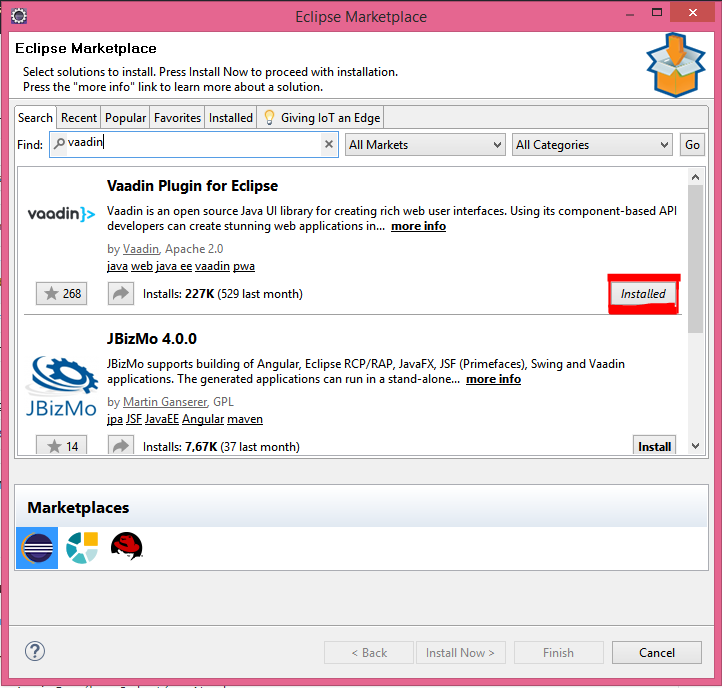
\includegraphics[width=0.5\textwidth]{img/Plugin_Vaadin}
\caption{Plugin Vaadin}\label{img:Vaadin}
\end{figure}

\section{Compilación, instalación y ejecución del proyecto}
Se explicará como compilar, instalar e ejecutar el proyecto. En el caso de la ejecución, se detallará como hacerlo con el términal de Windows y mediante Eclipse (IDE).

\subsection{Descarga del código fuente}
El código fuente se encuentra en el \href{https://github.com/dbo1001/Gestor-TFG-2016}{repositorio del proyecto} en GitHub. Para descargarlo se deberá hacer click en ``\textbf{\textit{Code}}'' y copiar la URL que se enseña en el apartado de HTTP. Con esta URL deberemos ir al GitHub Desktop y clonar el repositorio.

\imagen{GitHub_Code}{Copiar URL repositorio}

Para tener el código en local se deberá descargar el zip  ``\textbf{\textit{Download ZIP}}'' en la opción ``\textbf{\textit{Code}}'' anteriormente mencionada. Una vez descargado el zip se descomprimirá y abrirá con Eclipse. 
Para abrir el proyecto con eclipse se seleccionara en la barra de herramientas \textbf{\textit{File/Import\dots}}. Aparecerá una ventana en la que se optará por la opción ``\textbf{\textit{Projects from Folder or Archieve}}'' y se hará click en ``\textbf{\textit{Next}}''.

Después se hará click en ``\textbf{\textit{Directory\dots}}'' y se seleccionará la carpeta del proyecto con nombre sistinf y términaremos la importación con ``\textbf{\textit{Finish}}''.

\section{Pruebas del sistema}

\apendice{Documentación de usuario}

\section{Introducción}

\section{Requisitos de usuarios}

\section{Instalación}
No se requiere ninguna instalación por parte del usuario, simplemente puede acceder a la aplicación web a través del enlace \url{}.

\section{Manual del usuario}





\bibliographystyle{plain}
\bibliography{bibliografiaAnexos}

\end{document}
